\chapter{刚体}
\problem{已知方阵的矩阵对数由$\ln({1+M})=M-\frac12M^2+\frac13M^3-\cdots$定义. 
    \begin{enumerate}[label=(\arabic*)]
        \item 给定同阶方阵$X,Y$, 证明矩阵指数$\me^{X}\me^{Y}=\me^{Z}$由所谓Baker-Campbell-Hausdorff公式给出, 即$Z=X+Y+\frac{1}{2}[X,Y]+\frac{1}{12}[X,[X,Y]]-\frac{1}{12}[Y,[X,Y]]+\cdots$. \label{prob:12.1.1}
        \item 仿照\ref{prob:12.1.1}的推导, 利用无穷小三维转动生成元的对易式求$\me^{-\psi J_3}\me^{-\theta J_1}\me^{-\phi J_3}=\me^{\phi^1J_1+\phi^2J_2+\phi^3J_3}$的$\phi^1,\phi^2,\phi^3$, 精确到2阶.
    \end{enumerate}
}
\begin{solution}
    \begin{enumerate}[label=(\arabic*)]
        \item 把$\me^{X},\me^{Y}$展开到3阶即可. 
            \begin{align*}
                \me^{X}\me^{Y}&=(1+X+\frac12X^2+\frac16X^3)(1+Y+\frac12Y^2+\frac16Y^3)\\&=
                1+X+\frac12X^2+\frac16X^3+Y+\frac12Y^2+\frac16Y^3+XY+\frac12X^2Y+\frac12XY^2
            \end{align*}
            \begin{align*}
                \ln(\me^{X}\me^{Y})&=X+Y+\frac12(X^2+Y^2+2XY)+\frac16(X^3+Y^3+3X^2Y+3XY^2+Y^3)-\\&\frac12(X+Y+\frac12(X^2+Y^2+2XY))^2+\frac13(X+Y)^3\\&=X+Y+\frac12(X^2+Y^2+2XY)+\frac16(X^3+Y^3+3X^2Y+3XY^2+Y^3)-\\&\frac12\Big(X^2+Y^2+XY+YX+\frac12((X+Y)(X^2+Y^2+2XY)+(X^2+Y^2+2XY)(X+Y))\Big)\\&+\frac13(X^3+Y^2X+XYX+YX^2+X^2Y+Y^3+XY^2+YXY)\\&=X+Y+\frac12(XY-YX)-\frac14(2X^3+2Y^3+2YXY+2XYX+3X^2Y+3XY^2+Y^2X+YX^2)\\&+\frac16(X^3+3X^2Y+3XY^2+Y^3)+\frac13(X^3+Y^2X+XYX+YX^2+X^2Y+Y^3+XY^2+YXY)\\&=X+Y+\frac{1}{2}[X,Y]+\frac{1}{12}[X,[X,Y]]-\frac{1}{12}[Y,[X,Y]]
            \end{align*}
        \item 要求是展开到2阶, 那么只需要取前两项. 
        根据SO(3)生成元之间的对易关系$[J_i,J_j]=\varepsilon_{ijk}J_k$
        $$\me^{-\psi J_3}\me^{-\theta J_1}=\me^{-\psi J_3+-\theta J_1+\frac12\psi\theta J_2}$$
        而
        \begin{align*}
            \me^{-\psi J_3}\me^{-\theta J_1}\me^{-\phi J_3}&=\me^{-\psi J_3-\theta J_1+\frac12\psi\theta J_2}\me^{-\phi J_3}\\&=\me^{-\psi J_3-\theta J_1+\frac12\psi\theta J_2-\phi J_3-\frac12[\psi J_3+\theta J_1-\frac12\psi\theta J_2, \phi J_3]}\\&=\me^{-\psi J_3-\theta J_1+\frac12\psi\theta J_2-\phi J_3-\frac12\theta\phi J_2}
        \end{align*}
        也就是说$\phi^1=-\theta,\phi^2=\frac{1}{2}(\psi-\phi)\theta,\phi^3=-\psi-\phi$.
    \end{enumerate}
\end{solution}

\problem{求质量为$m$的匀质椭球$\frac{x^2}{a^2}+\frac{y^2}{b^2}+\frac{z^2}{c^2}=1$的相对于质心的转动惯量张量}
\begin{solution}
    采用广义球坐标换元$x=ar\sin\theta\cos\phi=ax_1,y=br\sin\theta\sin\phi=by_1,z=cr\cos\theta=cz_1$, 则容易看出$r$从0变化到1, 且$r=1$时$x,y,z$满足椭球方程. 
    其体积元写为$\dd V=abcr^2\sin\theta\,\dd r\,\dd \theta\,\dd \phi=abc\,\dd x'\dd y'\dd z'$
    
    由于
    $$\int_{x_1^2+y_1^2+z_1^2\leq1}(x_1^2+y_1^2+z_1^2)\dd x_1\dd y_1\dd z_1=\int_{r_1^2\leq1}r_1^2\times r_1^2\dd r_1\times4\pi$$
    立刻得到
    $$\int_{r_1^2\leq1}x_1^2\dd x_1\dd y_1\dd z_1=\frac{4\pi}{15}$$
    由于球的密度$\rho=\frac{m}{\frac43\pi abc}$
    所以计算积分
    $$\int_{\frac{x^2}{a^2}+\frac{y^2}{b^2}+\frac{z^2}{c^2}\leq1}\rho x^2\dd x\,\dd y\,\dd z=\frac{3}{4\pi}a^2m\int_{r_1^2\leq1}x_1^2\dd x_1\dd y_1\dd z_1=\frac{1}{5}ma^2$$
    因此可以得到
    $$I_{xx}=\frac15m(b^2+c^2), I_{yy}=\frac15m(a^2+c^2), I_{zz}=\frac15m(a^2+b^2)$$
    非对角元都是0. 
\end{solution}
\problem{证明刚体惯量张量三个对角元中任意一个不会大于另外两个之和.}
\begin{solution}
    直接计算即可
    \begin{align*}
        I_{xx}+I_{yy}-I_{zz}&=\int \rho(y^2+z^2+x^2+z^2-x^2-y^2)\dd \tau\\&=2\int\rho z^2 \,\dd \tau\geq0
    \end{align*}
\end{solution}
\problem{考虑例12.4中的立方体. 
    \begin{enumerate}[label=(\arabic*)]
        \item 求其相对质心基矢垂直于立方体表面的本体系中惯量张量;
        \item 证明以质心为原点的任意本体坐标系均为其惯量主轴, 并由此说明当质心绕定点转动时, 匀质立方体和匀质球不可分辨.
    \end{enumerate}
}
\begin{solution}
    由于对称性可以知道其三个对角元素均为相同的, 而非对角元均为0, 仅计算一个即可
    $$I_{xx}=\int\frac{m}{a^3}(y^2+z^2)\dd x\,\dd y\,\dd z=\frac16ma^2$$
    由于其转动惯量张量写为
    $$\begin{pmatrix}
        \frac16ma^2&0&0\\
        0&\frac16ma^2&0\\
        0&0&\frac16ma^2
    \end{pmatrix}=\frac16ma^2\cdot I$$
    其中$I$是单位矩阵, 在正交变换下具有不变性
    $$I'=RIR^{-1}=RR^{-1}=I,$$
    因此其转动惯量张量在任何正交归一坐标系下形式不变, 也易知动能与绕质心转动球相同, 而动能一样运动自然一样. 
\end{solution}
\problem{求例11.5中圆盘相对于质心角动量在本体坐标系中分量形式}
\begin{solution}
    本体坐标系下角速度为
    $$\vec{\omega}=\omega\frac{R}{L}\cos\phi\,\h{e}_1+\omega\frac{R}{L}\sin\phi\,\h{e}_2-\omega\, \h{e}_3$$
    由于其转动惯量张量为
    $$\begin{pmatrix}
        \frac14mR^2&0&0\\0&\frac14mR^2&0\\0&0&\frac14mR^2
    \end{pmatrix}$$
    得到其角动量
    $$\vec{L}=\frac14m\omega\frac{R^3}{L}\cos\phi \,\h{e}_1+\frac{1}{4}m\omega\frac{R^3}{L}\sin\phi \,\h{e}_2-\frac12mR^2\omega\,\h{e}_3$$
\end{solution}
\problem{如图\ref{fig:12-14}所示, 一个宽为$l$高为$h$的门板绕着一边以角速度$\omega$匀速旋转, 建立如图的本体系$\{\h{e}_i\}$,
    \begin{enumerate}[label=(\arabic*)]
        \item 求门板相对于O点的角动量在$\{\h{e}_i\}$中的分量;
        \item 为了维持门的旋转, 需要施加的相对于O点的扭矩.
    \end{enumerate}}
\begin{figure}[h]
    \centering
    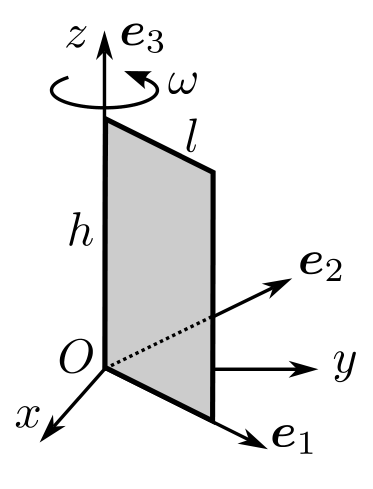
\includegraphics[width=0.2\textwidth]{content/Figures/12-14}
    \caption{ }
    \label{fig:12-14}
\end{figure}

\begin{solution}
    先求解相对于质心的角动量. 
    容易计算出其本体坐标系中的惯量张量为
    $$\begin{pmatrix}
        \frac{1}{12}mh^2&0&0\\0&\frac{1}{12}m(h^2+l^2)&0\\0&0&\frac{1}{12}ml^2
    \end{pmatrix}$$
    于是其相对于质心的角动量为
    $$\vec{L}_r=\frac{1}{12}ml^2\omega \,\h{e}_3$$
    再考虑质心相对于O点的角动量
    $$\vec{L}_c=m\vec{r}\times\vec{v}=\frac14m\omega l^2\,\h{e}_3-\frac14m\omega hl\,\h{e}_1$$
    熟知相对于O点角动量等于两项之和
    $$\vec{L}=\frac13m\omega l^2\,\h{e}_3-\frac14m\omega hl\,\h{e}_1$$
    当然可以直接计算其相对于O点的惯量张量. 
    $$I_{11}=\frac13mh^2,I_{22}=\frac13m(h^2+l^2),I_33=\frac13mh^2$$
    以及
    $$I_{13}=I_{31}=-\int\rho xz\dd x\,\dd z=-\frac14mhl$$
    再利用角动量公式$\vec{L}=\vec{I}\vec{\omega}$得到一样的结果. 
    由熟知公式
    $$\Big(\frac{\dd}{\dd t}\Big)_{\text{space}}=\Big(\frac{\dd}{\dd t}\Big)_{\text{body}}+\vec{\omega}\times$$
    得到力矩
    $$\vec{M}=\vec{\omega}\times\vec{L}=\frac14mhl\omega^2$$
\end{solution}
\problem{若自由刚体定点转动的角速度沿着某个主轴方向, 则被称为匀速转动. 
    \begin{enumerate}[label=(\arabic*)]
        \item 证明任意自由刚体都有匀速转动解;
        \item 设初始角速度沿着$\h{e}_1$方向, 刚体收到小扰动, 角速度变为$\omega_i\to\omega_i+\delta\omega_i$,求$\delta\omega_i$满足的微分方程并写成小振动方程的形式. \label{prob:12.7.2}
        \item 设刚体的主轴转动惯量为$I_1<I_2<I_3$, 利用\ref{prob:12.7.2}的结果, 证明刚体沿着最小和最大转动惯量对应的主轴的匀速转动是稳定的, 而沿着中间转动惯量对应的主轴的转动是不稳定的.
    \end{enumerate}}
\begin{solution}
    \begin{enumerate}[label=(\arabic*)]
        \item 只需要$\omega_1=C,\omega_2=\omega_3=0$或与其类似即可满足欧拉动力学方程.
        \item 由题知道角速度为
        $$\vec{\omega}=(\omega_1+\delta\omega_1)\,\h{e}_1+\delta\omega_2\,\h{e}_2+\delta\omega_3\,\h{e}_3$$
        由自由转动时三个欧拉动力学方程
        \begin{align*}
            I_1\dot{\delta\omega_1}&=\delta\omega_2\delta\omega_3(I_2-I_3)\\
            I_2\dot{\delta\omega_2}&=\delta\omega_3(\omega_1+\delta\omega_1)(I_3-I_1)\\
            I_3\dot{\delta\omega_3}&=(\omega_1+\delta\omega_1)\delta\omega_2(I_1-I_2)
        \end{align*}
        知道, 由于$\delta\omega_2,\delta\omega_3$都是小量, $\delta\omega_1$可以忽略. 
        因此原运动方程化为2元的
        \begin{align}
            I_2\dot{\delta\omega_2}&=\delta\omega_3\omega_1(I_3-I_1)\\
            I_3\dot{\delta\omega_3}&=\omega_1\delta\omega_2(I_1-I_2)
        \end{align}
        在(2)两边求导后带入(1)得到关于$\delta\omega_3$的二阶线性微分方程
        $$\ddot{\delta\omega_3}+\frac{(I_2-I_1)(I_3-I_1)}{I_2I_3}\omega_1^2\delta\omega_3=0$$
        同样可以得到
        $$\ddot{\delta\omega_2}+\frac{(I_2-I_1)(I_3-I_1)}{I_2I_3}\omega_1^2\delta\omega_2=0$$
        其假如存在小振动解, 本征频率为$\Omega=\sqrt{\frac{(I_2-I_1)(I_3-I_1)}{I_2I_3}}\omega_1$
        \item 假如初始绕着$2$轴旋转, 知道其本征频率为$\Omega=\sqrt{\frac{(I_1-I_2)(I_3-I_2)}{I_1I_3}}\omega_2$
        但是$I_1<I_2<I_3$, 所以根号下小于$0$, 对应解指数发散, 即不稳定.
    \end{enumerate}
\end{solution}

\problem{设对称陀螺相对质心的主轴转动惯量为$I_1=I_2=\lambda I_3$, 若陀螺绕质心自由转动, 初始章动角为$\theta_0$, 证明进动角速度$\dot{\psi}$与自转角速度$\dot{\varphi}$满足$\dot\psi=(\lambda-1)\dot\phi\cos\theta_0$}
\begin{solution}
    这题还是用欧拉动力学方程. 
    由于$I_1=I_2$, 立刻得到$\omega_3=C$
    由此得到关于$\omega_1,\omega_2$的方程
    \begin{align*}
        \lambda\dot{\omega_1}&=\omega_2\omega_3(\lambda-1)\\
        \lambda\dot{\omega_2}&=\omega_2\omega_3(-\lambda+1)
    \end{align*}
    因此解得
    $$\omega_1=A\cos(\frac{\lambda-1}{\lambda}\omega_3 t+\varphi),\omega_1=A\sin(\frac{\lambda-1}{\lambda}\omega_3 t+\varphi)$$
    也就是说, 有守恒量$\omega_1^2+\omega_2^2=C$
    于是可以知道总角动量大小守恒, 因为
    $$L^2=\lambda^2 I_3^2(\omega_1^2+\omega_2^2)+I_3^2\omega_3^2$$
    正文中已经给出, z轴角动量分量$p_\psi$也守恒, 即
    $$\cos\theta=\frac{p_\psi}{L}=\cos\theta_0$$
    为常数!
    由欧拉运动学方程得到
    $$\omega_1^2+\omega_2^2=\sin^2\theta\dot\phi^2+\dot\theta^2=C'$$
    即$\dot\phi=\frac{A}{\sin\theta_0}$是一个常数
    
    但是由于$$L^2=\lambda^2I_3^2(\omega_1^2+\omega_2^2)+I_3^2\omega_3^2=\lambda^2 I_3^2(\omega_1^2+\omega_2^2)+L^2\cos^2\theta$$
    于是可以得到
    $$\dot\phi=\frac{L}{\lambda I_3}$$
    由于$p_\psi=L\cos\theta=I_3(\dot\psi+\dot\phi\cos\theta_0)$
    解得
    $$\dot\psi=\frac{L(\lambda-1)}{I_3\lambda}\cos\theta_0$$
    即得到题给式子
    $$\dot\psi=(\lambda-1)\dot\phi\cos\theta_0$$
\end{solution}
